\documentclass[11pt]{article}
% Language setting
% Replace `english' with e.g. `spanish' to change the document language
\usepackage[english]{babel}


% Set page size and margins
% Replace `letterpaper' with `a4paper' for UK/EU standard size
\usepackage[a4paper,top=3cm,bottom=3cm,left=2.2cm,right=2.2cm, marginparwidth=0.5cm]{geometry}

% Useful packages
\usepackage[utf8]{inputenc}

% Font setup with fontspec
\usepackage{fontspec}

\setmonofont{Fira Code}[Scale=0.9]

% Header setup (Format 2: Title with Section)
\usepackage{fancyhdr}
\pagestyle{fancy}
\fancyhead{}
\fancyhead[L]{S2 Advanced Statistical Methods Coursework}
\fancyhead[R]{\rightmark}
\fancyfoot[C]{\thepage}
\renewcommand{\headrulewidth}{0.4pt}
\renewcommand{\sectionmark}[1]{\markright{#1}}

\usepackage{array}
\usepackage[most]{tcolorbox} % for inline code
\usepackage{amsmath}
\usepackage{graphicx}
\usepackage{caption}
\usepackage{subfigure}
\usepackage[colorlinks=true, allcolors=blue]{hyperref}
\usepackage{authblk}
\usepackage{amssymb}
\usepackage{listings}
\usepackage{color}
\usepackage{xcolor}
\usepackage{float}
\usepackage{biblatex} %Imports biblatex package
\addbibresource{references.bib} %Import the bibliography file
\usepackage{wrapfig}
\usepackage{booktabs}
\usepackage{longtable}
\usepackage{pdflscape}
\usepackage{booktabs}
\usepackage{multirow}
\usepackage{makecell}
\usepackage[british]{datetime2}

\renewcommand{\floatpagefraction}{0.1}
\renewcommand{\textfraction}{0}

\definecolor{dkgreen}{rgb}{0,0.6,0}
\definecolor{gray}{rgb}{0.5,0.5,0.5}
\definecolor{mauve}{rgb}{0.58,0,0.82}
\definecolor{lightgray}{gray}{0.9}
\definecolor{softorange}{RGB}{254, 236, 220}
\definecolor{reddishbrown}{RGB}{183, 69, 25}

\lstdefinestyle{pythonstyle}{
  language=Python,
  frame=tb,
  aboveskip=3mm,
  belowskip=3mm,
  showstringspaces=false,
  columns=flexible,
  basicstyle={\ttfamily\small},
  numbers=left,
  numberstyle=\tiny\color{gray},
  keywordstyle=\color{blue},
  commentstyle=\color{green!50!black},
  stringstyle=\color{red!70!black},
  breaklines=true,
  breakatwhitespace=true,
  tabsize=4,
  captionpos=b,
  morekeywords={self, cls, __init__, None},
}

\lstdefinestyle{pseudocode}{frame=tb,
  language=Python,
  aboveskip=3mm,
  belowskip=3mm,
  showstringspaces=false,
  columns=flexible,
  basicstyle={\small\ttfamily},
  numbers=left,
  numberstyle=\tiny\color{gray},
  keywordstyle=\color{blue},
  commentstyle=\color{dkgreen},
  stringstyle=\color{mauve},
  breaklines=true,
  breakatwhitespace=true,
  tabsize=3
}

\lstdefinestyle{input}{frame=none,
  aboveskip=3mm,
  belowskip=3mm,
  showstringspaces=false,
  columns=flexible,
  basicstyle={\small\ttfamily},
  numbers=none,
  numberstyle=\tiny\color{gray},
  keywordstyle=\color{blue},
  commentstyle=\color{dkgreen},
  stringstyle=\color{mauve},
  breaklines=true,
  breakatwhitespace=true,
  tabsize=3,
  captionpos=b,
}


\definecolor{notebackground}{RGB}{250, 244, 237}
\definecolor{notetextgray}{RGB}{60, 60, 60}

\lstdefinestyle{notebookoutput}{
    backgroundcolor=\color{notebackground},
    basicstyle=\ttfamily\small\color{notetextgray},
    frame=none,
    xleftmargin=1.5em,
    showstringspaces=false,
    numbers=none,
    breaklines=true,
    postbreak=\mbox{\textcolor{gray}{$\hookrightarrow$}\space},
}

% inline code display
\newtcbox{\inlinecode}{
  nobeforeafter,
  colback=softorange,
  colframe=white,
  boxrule=0pt,
  arc=1mm,
  left=0pt, right=0pt, top=0pt, bottom=0pt,
  on line,
  fontupper=\scriptsize\ttfamily\color{reddishbrown}
}


% make title
\title{
\includegraphics[scale=0.2]{Cam_logo_bw.png}\\
\vspace{0.5cm}
S2 Advanced Statistical Methods Coursework
}
\author{xl628}
\affil{Department of Physics}

\begin{document}

\maketitle

\vspace{1cm}
\noindent
\textbf{Document Statistics:} \\
Words in text: 2085 \\
Words in headers: 64 \\
Words outside text (captions, etc.): 538 \\

\section{Introduction}

The Antikythera mechanism is an ancient Greek astronomical device that incorporated a perforated calendar ring. Although only a quarter of this ring survives—and is fractured and misaligned—its original function and structure remain subjects of debate. Earlier interpretations proposed a 365-hole solar calendar, but more recent analysis suggests a 354-hole lunar calendar \cite{budiselic2021antikythera}. In this report, we use hole location data from \cite{thoeni2019replication} and statistical modelling to estimate the original number of holes, accounting for both translations and rotations of the fragmented sections.


\begin{figure}[h!]
\centering

\includegraphics[width=0.85\textwidth]{./figures/hole_locations.pdf}
\caption{Hole positions on the Antikythera mechanism's calendar ring. Coloured points represent 81 measured hole locations across eight distinct sections (0–7). Coordinates of each hole centre are given in millimetres. Section IDs are defined by physical cracks.}
\label{fig:hole_locations}
\end{figure}

\section{Model}

The model we employ is introduced in \cite{woan2024improvedcalendarringholecount}. It accounts for both translational and rotational displacements of the fragmented sections relative to their original positions.

\subsection{Hole Measurement Data}

The measured hole locations $\mathbf{d}_i \in \mathbb{R}^2$ in the $x$-$y$ plane are shown in Figure \ref{fig:hole_locations}, where $i = 1, \ldots, 81$ labels the holes. Each hole belongs to a section (fragment), labelled $j = 0, \ldots, 7$.



\subsection{Model for Hole Locations}


The three models considered are nested and based on a common Gaussian error assumption. The ideal and isotropic models are specific cases of the more general radial-tangential model.

\paragraph{Ideal Hole Positions}
\label{sec:ideal}
In an ideal, undamaged ring with $N$ holes, the holes would be arranged in a perfect circle with radius $r$. The angular position of the $i$-th hole (where $i = 1, 2, \ldots, N$ would be:
$$\theta_i = 2\pi \frac{(i-1)}{N} + \theta_0$$
where $\theta_0$ is the initial phase for the observed data.

The corresponding Cartesian coordinates are:
 $\mathbf{m}_i^{\text{ideal}}=\mathbf{r}_0+\mathbf{r}_i = \left(x_0+r \cos(\theta_i), y_0 + r \sin(\theta_i)\right)$
where $\mathbf{r}_0 = (x_0, y_0)$ is the centre of the ring.

\paragraph{Fragmented Ring with Displaced Sections}

In reality, we observe a fragmented ring composed of $s$ arc sections (labelled $j = 0, 1, \ldots, s-1$), each subject to its own translation and rotation. The centre of the $j$-th section is located at $\mathbf{r}_{0j} = (x_{0j}, y_{0j})$, and the section has a rotational offset $\alpha_j$.


For the $i$-th hole in the $j$-th section, the angular position is:

$$\phi_{ij} = 2\pi \frac{(i-1)}{N} + \alpha_j$$

And its Cartesian coordinates $\mathbf{m}_{i}^{\text{sectioned}}=\mathbf{r}_{0j} + \mathbf{r}_{ij}=(x_{ij},y_{ij})$ are:

$$x_{ij} = x_{0j} + r \cos(\phi_{ij})$$
$$y_{ij} = y_{0j} + r \sin(\phi_{ij})$$

where $\mathbf{r}_{ij}$ represents the intended position of the $i$-th hole in section $j$, relative to the centre of its arc.


\subsection{Likelihood Functions}

We assume that the errors in hole measurement and placement follow a 2D isotropic Gaussian distribution.

\paragraph{Isotropic Model}
In the isotropic model, the covariance matrix is:

$$\Sigma = \begin{pmatrix} \sigma^2 & 0 \\ 0 & \sigma^2 \end{pmatrix}$$

Given a measured hole position $\mathbf{d}_i = (x_i, y_i)$ and the corresponding model prediction $\mathbf{m}_i = (x_{ij}, y_{ij})$, the likelihood is:

$$\mathcal{L}(\mathbf{d}_i \mid \boldsymbol{\theta}) = \frac{\exp \left(-\frac{1}{2\sigma^2}\|\mathbf{d}_i - \mathbf{m}_i\|^2\right)}{2\pi\sigma^2}$$
Here, $\boldsymbol{\theta}$ represents all model parameters: $(N, r, \sigma, {(x_{0j}, y_{0j}, \alpha_j)})$.

The log-likelihood for a single hole is:

$$\log \mathcal{L}(\mathbf{d}_i \mid \boldsymbol{\theta}) = -\frac{1}{2\sigma^2}\|\mathbf{d}_i - \mathbf{m}_i\|^2 - \log(2\pi\sigma^2)$$

And the total log-likelihood for all $n$ holes is:

\begin{equation}
\label{eq:ml_isotropic}
    \log \mathcal{L}(\{\mathbf{d}_i\} \mid \boldsymbol{\theta}) = -\frac{1}{2\sigma^2}\sum_{i=1}^{n}\|\mathbf{d}_i - \mathbf{m}_i\|^2 - n\log(2\pi\sigma^2)
\end{equation}

\paragraph{Radial-Tangential Model}


In the radial-tangential model, we assume that the errors in hole placement differ in magnitude between the radial and tangential directions.

For each hole, we define radial and tangential unit vectors:

\begin{equation}
\label{eq:r_t_unit}
\begin{aligned}
    \hat{\mathbf{r}}_{ij} &= (\cos\phi_{ij}, \sin\phi_{ij}) \\
    \hat{\mathbf{t}}_{ij} &= (\sin\phi_{ij}, -\cos\phi_{ij})
\end{aligned}
\end{equation}

The error vector $\mathbf{e}_{ij} = \mathbf{m}_i - \mathbf{d}_i$ can be projected onto these directions:

$$e_r = \mathbf{e}_{ij} \cdot \hat{r}_{ij}$$
$$e_t = \mathbf{e}_{ij} \cdot \hat{t}_{ij}$$

The covariance matrix in the radial/tangential coordinate system is:

$$C = \begin{pmatrix} \sigma_r^2 & 0 \\ 0 & \sigma_t^2 \end{pmatrix}$$

The likelihood for a single hole is:

$$\mathcal{L}(\mathbf{d}_i \mid \boldsymbol{\theta}) = \frac{\exp \left(-\frac{1}{2}\left[\frac{e_r^2}{\sigma_r^2} + \frac{e_t^2}{\sigma_t^2}\right]\right)}{2\pi\sigma_r\sigma_t}$$

And the log-likelihood is:

$$\log \mathcal{L}(\mathbf{d}_i \mid \boldsymbol{\theta}) = -\frac{1}{2}\left[\frac{e_r^2}{\sigma_r^2} + \frac{e_t^2}{\sigma_t^2}\right] - \log(2\pi\sigma_r\sigma_t)$$

The total log-likelihood for all holes is:

\begin{equation}
\label{eq:ml_rt}
    \log \mathcal{L}(\{\mathbf{d}_i\} \mid \boldsymbol{\theta}) = -\frac{1}{2}\sum_{i=1}^{n}\left[\frac{e_r^2}{\sigma_r^2} + \frac{e_t^2}{\sigma_t^2}\right] - n\log(2\pi\sigma_r\sigma_t)
\end{equation}


\begin{table}[h!]
\centering
\caption{Log-Likelihood and Derivatives for Isotropic and Radial-Tangential Models}
\begin{tabular}{>{\raggedright\arraybackslash}p{4cm} >{\raggedright\arraybackslash}p{10cm}}
\toprule
\textbf{Model Component} & \textbf{Expression} \\
\midrule
\multicolumn{2}{c}{\textbf{Isotropic Model}} \\
\midrule
Log-Likelihood &
$\log \mathcal{L} = -\frac{1}{2\sigma^2} \sum_{i=1}^n \|\mathbf{d}_i - \mathbf{m}_i\|^2 - n \log (2\pi \sigma^2)$, \\
& where $\|\mathbf{d}_i - \mathbf{m}_i\|^2 = (x_i - x_{ij})^2 + (y_i - y_{ij})^2$ \\
\midrule
$\frac{\partial \log \mathcal{L}}{\partial x_{0j}}$  &
$\frac{1}{\sigma^2} \sum_{i: j(i)=j} (x_i - x_{ij})$ \\
\midrule
$\frac{\partial \log \mathcal{L}}{\partial y_{0j}}$  &
$\frac{1}{\sigma^2} \sum_{i: j(i)=j} (y_i - y_{ij})$ \\
\midrule
$\frac{\partial \log \mathcal{L}}{\partial \alpha_j}$  &
$\frac{r}{\sigma^2} \sum_{i: j(i)=j} \left[ (y_i - y_{ij}) \cos \phi_{ij} - (x_i - x_{ij}) \sin \phi_{ij} \right]$ \\
\midrule
$\frac{\partial \log \mathcal{L}}{\partial r}$ &
$\frac{1}{\sigma^2} \sum_{i=1}^n \left[ (x_i - x_{ij}) \cos \phi_{ij} + (y_i - y_{ij}) \sin \phi_{ij} \right]$ \\
\midrule
$\frac{\partial \log \mathcal{L}}{\partial \sigma}$  &
$\frac{1}{\sigma^3} \sum_{i=1}^n \|\mathbf{d}_i - \mathbf{m}_i\|^2 - \frac{2n}{\sigma}$ \\
\midrule
$\frac{\partial \log \mathcal{L}}{\partial N}$ &
$\frac{2\pi r}{\sigma^2 N^2} \sum_{i=1}^n (i-1) \left[ (x_i - x_{ij}) \sin \phi_{ij} - (y_i - y_{ij}) \cos \phi_{ij} \right]$ \\
\midrule
\multicolumn{2}{c}{\textbf{Radial/Tangential Model}} \\
\midrule
Log-Likelihood &
$\log \mathcal{L} = -\frac{1}{2} \sum_{i=1}^n \left[ \frac{e_r^2}{\sigma_r^2} + \frac{e_t^2}{\sigma_t^2} \right] - n \log (2\pi \sigma_r \sigma_t)$, \\
& where $e_r = (\mathbf{m}_i - \mathbf{d}_i) \cdot \hat{\mathbf{r}}_{ij}$, $e_t = (\mathbf{m}_i - \mathbf{d}_i) \cdot \hat{\mathbf{t}}_{ij}$, \\
& $\hat{\mathbf{r}}_{ij} = (\cos \phi_{ij}, \sin \phi_{ij})$, $\hat{\mathbf{t}}_{ij} = (\sin \phi_{ij}, -\cos \phi_{ij})$ \\
\midrule
$\frac{\partial \log \mathcal{L}}{\partial x_{0j}}$ &
$\sum_{i: j(i)=j} \left[ \frac{e_r}{\sigma_r^2} \cos \phi_{ij} + \frac{e_t}{\sigma_t^2} \sin \phi_{ij} \right]$ \\
\midrule
$\frac{\partial \log \mathcal{L}}{\partial y_{0j}}$ &
$\sum_{i: j(i)=j} \left[ \frac{e_r}{\sigma_r^2} \sin \phi_{ij} - \frac{e_t}{\sigma_t^2} \cos \phi_{ij} \right]$ \\
\midrule
$\frac{\partial \log \mathcal{L}}{\partial \alpha_j}$ &
$\sum_{i: j(i)=j} \left[ \frac{e_r e_t}{\sigma_r^2} - \frac{e_t (r + e_r)}{\sigma_t^2} \right]$ \\
\midrule
$\frac{\partial \log \mathcal{L}}{\partial r}$ &
$\frac{1}{\sigma_r^2} \sum_{i=1}^n e_r$ \\
\midrule
$\frac{\partial \log \mathcal{L}}{\partial \sigma_r}$ &
$\frac{1}{\sigma_r^3} \sum_{i=1}^n e_r^2 - \frac{n}{\sigma_r}$ \\
\midrule
$\frac{\partial \log \mathcal{L}}{\partial \sigma_t}$ &
$\frac{1}{\sigma_t^3} \sum_{i=1}^n e_t^2 - \frac{n}{\sigma_t}$ \\
\midrule
$\frac{\partial \log \mathcal{L}}{\partial N}$ &
$-\frac{2\pi}{N^2} \sum_{i=1}^n (i-1) \left[ \frac{e_r e_t}{\sigma_r^2} - \frac{e_t (r + e_r)}{\sigma_t^2} \right]$ \\
\midrule
\multicolumn{2}{c}{\textbf{Notations}} \\
\midrule
Angular Position &
$\phi_{ij} = 2\pi \frac{(i-1)}{N} + \alpha_j$ \\
\midrule
Cartesian Coordinates &
$\mathbf{m}_{i} = \mathbf{r}_{0j} + \mathbf{r}_{ij} = (x_{ij}, y_{ij})$, \\
& where $x_{ij} = x_{0j} + r \cos(\phi_{ij})$, $y_{ij} = y_{0j} + r \sin(\phi_{ij})$ \\
\midrule
Notation $i: j(i)=j$ &
The index $i$ runs over all holes such that hole $i$ belongs to arc section $j$ \\
\bottomrule
\end{tabular}
\label{tab:ll}
\end{table}



\section{Gradient Computation}

For optimisation and Hamiltonian Monte Carlo (HMC) sampling, we require the gradients of the log-likelihood functions with respect to the model parameters.

We define the operations in the model using \inlinecode{jax.numpy}.

Maximum Likelihood estimates are computed using \inlinecode{scipy.optimize.minimize}, with gradients supplied to enhance optimisation performance. These gradients are obtained via \inlinecode{jax.grad}.


For HMC sampling, we utilise the \inlinecode{numpyro} library in combination with JAX-based \cite{jax2018github} automatic differentiation. This approach works by building the computational graph of the function and applying the chain rule to compute derivatives with respect to all parameters.

The analytical forms of the derivatives are also derived and used to validate the model implementation, with tests provided in \texttt{tests/model\_test.py}. A summary of the log-likelihood expressions and their corresponding derivatives is presented in Table \ref{tab:ll}.

The tests evaluate the gradient values at a point in the parameter space (near our optimisation results) for each model, with both absolute and relative error tolerances set to $1\times 10^{-4}$. When the evaluation point is changed, most gradients remain within this threshold; however, a few cases—often involving the $\alpha$ parameters—exceed it.

Due to the complexity of these derivatives and considerations of efficiency, we rely on automatic differentiation (via JAX) in the implementation rather than computing the gradients manually.







\section{Maximum Likelihood Estimates}

This section is primarily implemented in the notebook \texttt{02\_maximum\_likelihood.ipynb}.

\subsection{Model Fitting}
We begin by fitting the ideal model described in Section~\ref{sec:ideal}, using its results as initial values for the subsequent sectioned models. Optimisation of the negative log-likelihoods is performed using the \inlinecode{"trust-constr"} and \inlinecode{"L-BFGS-B"} methods available in \inlinecode{scipy.optimize.minimize}.

To estimate uncertainties, we employ a non-parametric bootstrap procedure to generate 100 samples per model. For the ideal model, we resample the dataset with replacement. For the sectioned models, we resample hole indices within each section, again with replacement. Each sample maintains the same size as the original dataset (81 holes in total). The results are summarised in Tables~\ref{tab:bs-1} and~\ref{tab:bs-2}.




\begin{table}[ht]
\centering
\caption{Bootstrap results for different models. For each parameter, the median, mean ± standard deviation, and several confidence intervals (68\%, 90\%, 95\%, 99\%) are reported.}
\begin{tabular}{llrrrrrr}
\toprule
Model & Parameter & \multicolumn{1}{c}{Median} & \multicolumn{1}{c}{Mean $\pm$ Std} & \multicolumn{1}{c}{68\% CI} & \multicolumn{1}{c}{90\% CI} & \multicolumn{1}{c}{95\% CI} & \multicolumn{1}{c}{99\% CI} \\
\midrule
\multirow{6}{*}{Ideal} & $N$ & 356.645 & 356.544 $\pm$ 0.690 & $^{+0.480}_{-0.834}$ & $^{+1.057}_{-1.307}$ & $^{+1.238}_{-1.404}$ & $^{+1.461}_{-2.043}$ \\
 & $r$ & 78.320 & 78.298 $\pm$ 0.172 & $^{+0.143}_{-0.193}$ & $^{+0.280}_{-0.319}$ & $^{+0.299}_{-0.364}$ & $^{+0.346}_{-0.455}$ \\
 & $\sigma$ & 0.149 & 0.149 $\pm$ 0.009 & $^{+0.010}_{-0.009}$ & $^{+0.016}_{-0.013}$ & $^{+0.018}_{-0.016}$ & $^{+0.022}_{-0.020}$ \\
 & $x_0$ & 80.467 & 80.461 $\pm$ 0.078 & $^{+0.061}_{-0.089}$ & $^{+0.124}_{-0.142}$ & $^{+0.152}_{-0.157}$ & $^{+0.160}_{-0.199}$ \\
 & $y_0$ & 136.620 & 136.604 $\pm$ 0.166 & $^{+0.138}_{-0.184}$ & $^{+0.291}_{-0.304}$ & $^{+0.299}_{-0.346}$ & $^{+0.333}_{-0.437}$ \\
 & $\theta_0$ & 214.276 & 214.270 $\pm$ 0.065 & $^{+0.046}_{-0.075}$ & $^{+0.107}_{-0.116}$ & $^{+0.111}_{-0.133}$ & $^{+0.170}_{-0.190}$ \\
\midrule
\multirow{3}{*}{Isotropic} & $N$ & 357.395 & 357.399 $\pm$ 0.010 & $^{+0.008}_{-0.000}$ & $^{+0.019}_{-0.000}$ & $^{+0.023}_{-0.001}$ & $^{+0.060}_{-0.003}$ \\
 & $r$ & 77.923 & 77.921 $\pm$ 0.008 & $^{+0.003}_{-0.008}$ & $^{+0.008}_{-0.019}$ & $^{+0.009}_{-0.023}$ & $^{+0.010}_{-0.026}$ \\
 & $\sigma$ & 0.086 & 0.087 $\pm$ 0.005 & $^{+0.005}_{-0.004}$ & $^{+0.009}_{-0.007}$ & $^{+0.010}_{-0.008}$ & $^{+0.011}_{-0.010}$ \\
\midrule
\multirow{4}{*}{Radial-Tangential} & $N$ & 357.268 & 357.277 $\pm$ 0.035 & $^{+0.004}_{-0.001}$ & $^{+0.056}_{-0.002}$ & $^{+0.123}_{-0.005}$ & $^{+0.202}_{-0.008}$ \\
 & $r$ & 77.854 & 77.847 $\pm$ 0.030 & $^{+0.003}_{-0.005}$ & $^{+0.004}_{-0.046}$ & $^{+0.005}_{-0.128}$ & $^{+0.007}_{-0.160}$ \\
 & $\sigma_r$ & 0.025 & 0.025 $\pm$ 0.002 & $^{+0.003}_{-0.002}$ & $^{+0.004}_{-0.004}$ & $^{+0.004}_{-0.004}$ & $^{+0.005}_{-0.006}$ \\
 & $\sigma_t$ & 0.117 & 0.116 $\pm$ 0.008 & $^{+0.007}_{-0.007}$ & $^{+0.011}_{-0.014}$ & $^{+0.012}_{-0.018}$ & $^{+0.016}_{-0.025}$ \\
\bottomrule
\end{tabular}
\label{tab:bs-1}
\end{table}

\begin{table}[ht]
\centering
\caption{Bootstrap-derived, section-specific estimates of $x_0$, $y_0$, and $\alpha$ for the Isotropic and Radial–Tangential models. Reported values are medians with 68\% confidence intervals.}
\small
\begin{tabular}{clrrrr}
\toprule
Model & Section & \multicolumn{1}{c}{$x_0$ (Median)} & \multicolumn{1}{c}{$y_0$ (Median)} & \multicolumn{1}{c}{$\alpha$ (Median)} \\
\midrule
\multirow{8}{*}{Isotropic}
& Section 0 & 80.097 $^{+0.000}_{-0.003}$ & 136.372 $^{+0.000}_{-0.002}$ & 214.165 $^{+0.001}_{-0.002}$ \\
& Section 1 & 80.108 $^{+0.002}_{-0.015}$ & 136.473 $^{+0.001}_{-0.016}$ & 214.352 $^{+0.024}_{-0.021}$ \\
& Section 2 & 80.236 $^{+0.000}_{-0.004}$ & 136.206 $^{+0.001}_{-0.006}$ & 214.451 $^{+0.022}_{-0.020}$ \\
& Section 3 & 79.853 $^{+0.011}_{-0.001}$ & 136.291 $^{+0.011}_{-0.001}$ & 214.804 $^{+0.011}_{-0.014}$ \\
& Section 4 & 80.505 $^{+0.003}_{-0.000}$ & 136.469 $^{+0.001}_{-0.012}$ & 214.290 $^{+0.001}_{-0.001}$ \\
& Section 5 & 80.509 $^{+0.004}_{-0.000}$ & 136.488 $^{+0.001}_{-0.014}$ & 214.313 $^{+0.043}_{-0.039}$ \\
& Section 6 & 80.615 $^{+0.003}_{-0.000}$ & 136.189 $^{+0.001}_{-0.008}$ & 214.675 $^{+0.058}_{-0.059}$ \\
& Section 7 & 80.770 $^{+0.000}_{-0.011}$ & 136.048 $^{+0.032}_{-0.001}$ & 214.458 $^{+0.025}_{-0.040}$ \\
\midrule
\multirow{8}{*}{Radial-Tangential}
& Section 0 & 80.018 $^{+0.001}_{-0.004}$ & 136.318 $^{+0.001}_{-0.002}$ & 214.166 $^{+0.000}_{-0.001}$ \\
& Section 1 & 80.057 $^{+0.008}_{-0.038}$ & 136.399 $^{+0.017}_{-0.012}$ & 214.345 $^{+0.034}_{-0.041}$ \\
& Section 2 & 80.185 $^{+0.007}_{-0.009}$ & 136.154 $^{+0.013}_{-0.011}$ & 214.460 $^{+0.020}_{-0.024}$ \\
& Section 3 & 79.901 $^{+0.028}_{-0.024}$ & 136.231 $^{+0.006}_{-0.010}$ & 214.750 $^{+0.025}_{-0.026}$ \\
& Section 4 & 80.542 $^{+0.001}_{-0.000}$ & 136.319 $^{+0.001}_{-0.005}$ & 214.265 $^{+0.002}_{-0.002}$ \\
& Section 5 & 80.648 $^{+0.004}_{-0.002}$ & 136.421 $^{+0.005}_{-0.012}$ & 214.202 $^{+0.040}_{-0.041}$ \\
& Section 6 & 80.667 $^{+0.003}_{-0.001}$ & 136.105 $^{+0.004}_{-0.009}$ & 214.632 $^{+0.057}_{-0.059}$ \\
& Section 7 & 82.751 $^{+0.005}_{-0.003}$ & 136.793 $^{+0.009}_{-0.007}$ & 212.863 $^{+0.039}_{-0.039}$ \\
\bottomrule
\end{tabular}
\label{tab:bs-2}
\end{table}


Notably, the sectioned models yield lower bootstrap uncertainties for global parameters such as $N$, $r$, and $\sigma$, in comparison to the ideal model, which assumes a single shared circle centre across all sections.

Figure~\ref{fig:ml_fits} presents the observed and model-predicted hole positions, annotated with the corresponding negative log-likelihood (NLL) values.


\subsection{Model Comparison}
\label{sec:lrt}

Likelihood values provide a measure of how well a model fits the data, but they do not account for model complexity. As a result, more complex models may achieve higher likelihoods simply by overfitting noise rather than capturing true structure.


In this case, both the ideal and isotropic models are nested within the more general radial–tangential model.  This nesting allows us to apply a likelihood-ratio test (LRT) to determine whether the added complexity yields a statistically significant improvement in model fit.

The test statistic is defined as:

$$
\lambda = -2(\ln L_{\text{simple}} - \ln L_{\text{complex}}) = -2(160.04 - 235.51) = 150.94
$$

Under the null hypothesis (that the simpler \textbf{isotropic} model is sufficient), this test statistic approximately follows a $\chi^2$ distribution, with degrees of freedom equal to the difference in parameter count (1 in this case).

Comparing this value to the critical threshold from the \(\chi^2\) distribution:

\[
\lambda = 150.94 \gg \chi^2_{0.001,1} = 10.83
\]
we can reject the null hypothesis at $p < 0.001$. This provides extremely strong evidence that the radial–tangential model, with separate parameters $\sigma_r$ and $\sigma_t$, offers \textbf{a significantly improved fit} compared to the isotropic model.

\newpage
\begin{figure}[h!]
    \centering
    \subfigure[Ideal Circle Model, NLL = -77.11]{
        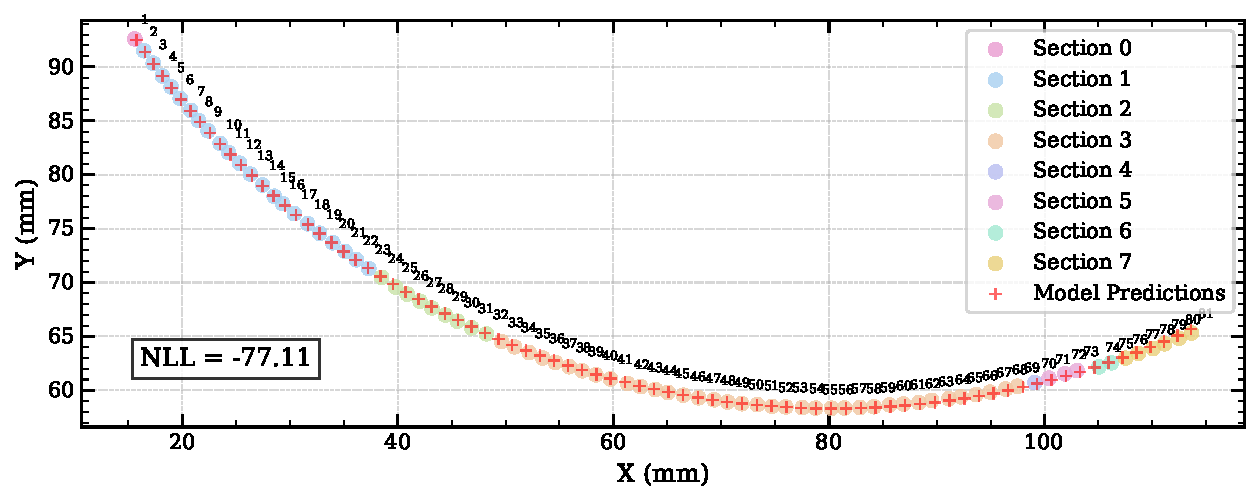
\includegraphics[width=0.9\textwidth]{./figures/ml_ideal_model.pdf}
        \label{fig:ml_ideal}
    }
    \subfigure[Isotropic Model, NLL = -160.04]{
        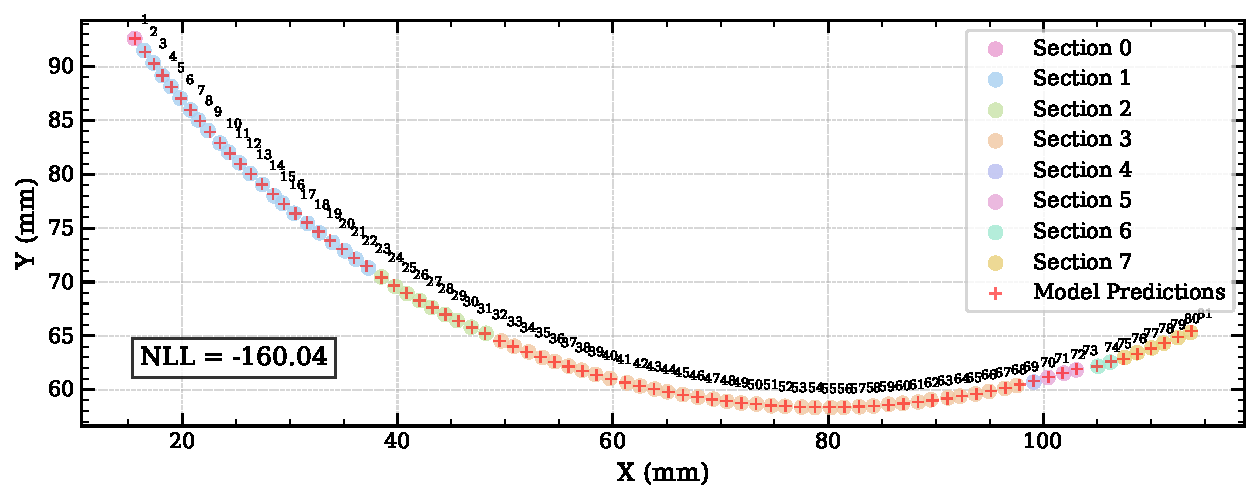
\includegraphics[width=0.9\textwidth]{./figures/ml_isotropic_model.pdf}
        \label{fig:ml_isotropic}
    }
    \subfigure[Radial-Tangential Model, NLL = -235.51]{
        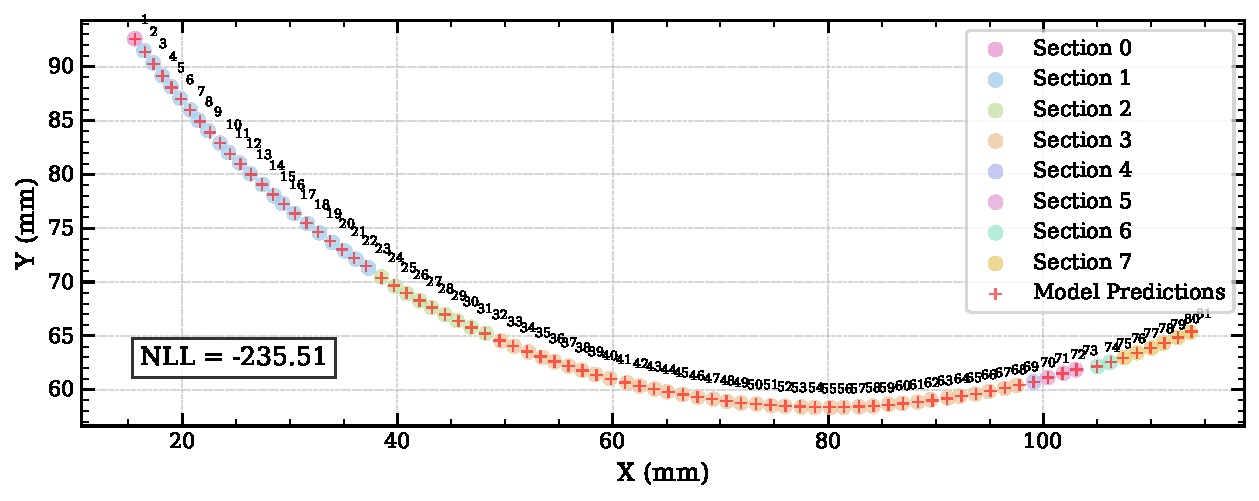
\includegraphics[width=0.9\textwidth]{./figures/ml_radial_tangential_model.pdf}
        \label{fig:ml_radial_tangential}
    }
    \caption{Maximum likelihood fits to the Antikythera mechanism's calendar ring hole positions. (a) The ideal circle model shows measured hole positions (coloured points) across eight sections (0–7), along with predicted positions (red crosses). (b) The isotropic model yields improved fit quality. (c) The radial–tangential model provides the best fit to the measured hole positions, as indicated by the lowest negative log-likelihood (NLL) value.}
    \label{fig:ml_fits}
\end{figure}
\newpage


\section{MCMC Sampling}

This section corresponds to the implementation in the notebook \texttt{03\_mcmc\_sampling.ipynb}.


\begin{figure}[h!]
    \centering
    \subfigure[Isotropic model]{
        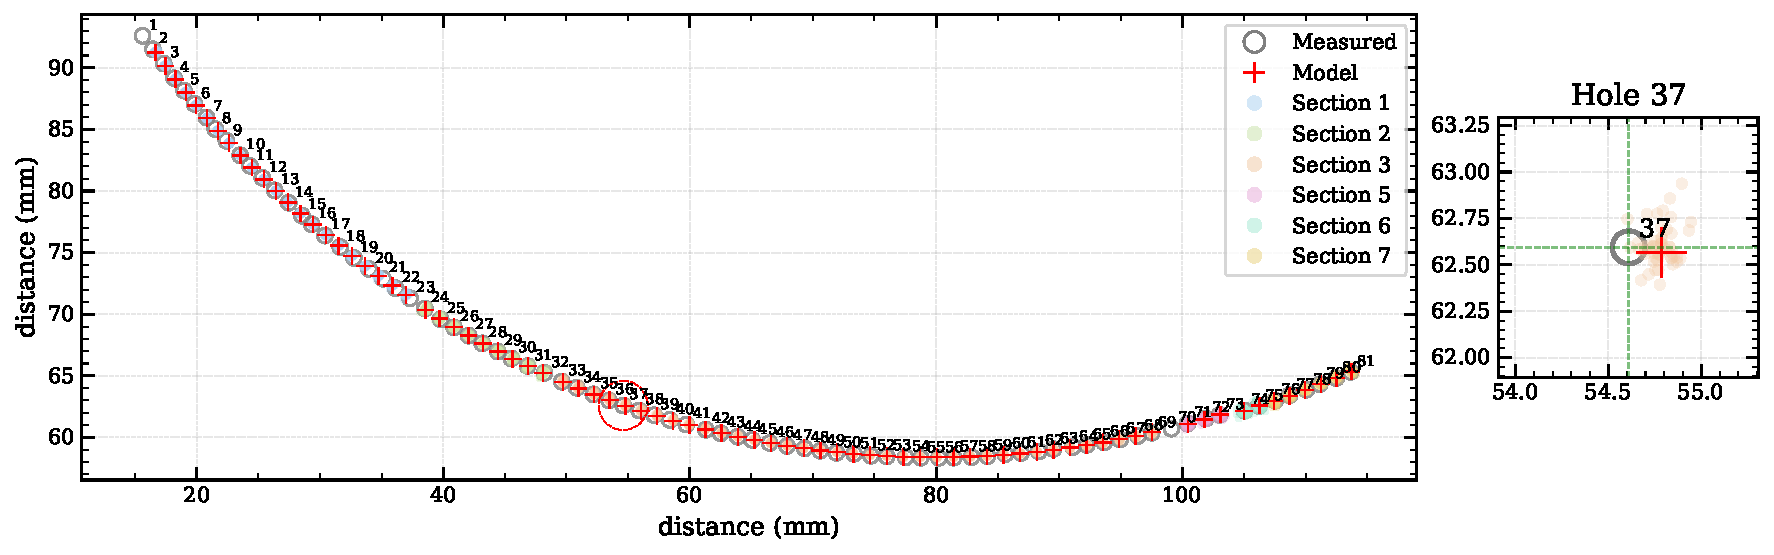
\includegraphics[width=0.99\textwidth]{./figures/isotropic_model.pdf}
        \label{fig:locations_isotropic}
    }
    \vspace{0.5cm}
    \subfigure[Radial-tangential model]{
        
\includegraphics[width=0.99\textwidth]{./figures/radial_tangential_model.pdf}
        \label{fig:locations_rt}
    }
    \caption{Measured and modelled hole positions on the Antikythera mechanism calendar ring under two fitted models. (a) Isotropic model: the left panel shows all measured hole positions (grey circles) and model predictions (red crosses) across fragments (coloured by section), annotated with hole numbers; the right panel magnifies Hole 37 to illustrate model uncertainty using 50 posterior samples from MCMC (coloured dots). The uncertainty is roughly circular due to the isotropic noise assumption. (b) Radial–tangential model: same layout as (a), but the uncertainty in Hole 37 is elongated along the tangential direction, reflecting anisotropic error structure. Sections 0 and 4 are excluded from both analyses.}
    \label{fig:locations_combined}
\end{figure}

\subsection{Model Fitting}

We employ the No-U-Turn Sampler (NUTS) implemented in \inlinecode{numpyro}\cite{phan2019composable,bingham2019pyro} to sample from the posterior distributions of the model parameters. NUTS is a variant of the Hamiltonian Monte Carlo (HMC) algorithm that automatically determines the number of steps to take during sampling, thereby avoiding inefficient “U-turns” in the sampling trajectory. We use uniform priors for all parameters, except for the noise parameters ($\sigma$ or $\sigma_r$, $\sigma_t$), which follow a Jeffreys prior (log-uniform).

In this implementation, we exclude sections with only a single data point (Sections 0 and 4). Conceptually, even when the radius $r$ is known, at least two points are required to uniquely determine the circle; otherwise, the centre coordinates and phase angle remain fundamentally underdetermined. Furthermore, including these sections significantly deteriorates the sampling performance. If their inclusion is essential, introducing hyperpriors over ${x_{0j}, y_{0j}, \alpha_{0j}}$ may help to stabilise the inference—although this extension is beyond the scope of the present report.

\begin{table}[ht]
\centering
\caption{Posterior summary statistics for global parameters in the isotropic and radial–tangential models obtained from MCMC sampling.}
\begin{tabular}{llrrrrrr}
\toprule
Model & Parameter & \multicolumn{1}{c}{Median} & \multicolumn{1}{c}{Mean $\pm$ Std} & \multicolumn{1}{c}{68\% CI} & \multicolumn{1}{c}{90\% CI} & \multicolumn{1}{c}{95\% CI} & \multicolumn{1}{c}{99\% CI} \\
\midrule
\multirow{3}{*}{Isotropic} & $N$ & 359.245 & 359.252 $\pm$ 1.034 & $^{+1.026}_{-1.013}$ & $^{+1.708}_{-1.677}$ & $^{+2.038}_{-2.011}$ & $^{+2.719}_{-2.669}$ \\
 & $r$ & 77.450 & 77.449 $\pm$ 0.203 & $^{+0.201}_{-0.203}$ & $^{+0.333}_{-0.331}$ & $^{+0.399}_{-0.400}$ & $^{+0.528}_{-0.535}$ \\
 & $\sigma$ & 0.338 & 0.339 $\pm$ 0.020 & $^{+0.021}_{-0.019}$ & $^{+0.035}_{-0.031}$ & $^{+0.042}_{-0.036}$ & $^{+0.057}_{-0.046}$ \\
\midrule
\multirow{4}{*}{Radial-Tangential} & $N$ & 358.507 & 358.521 $\pm$ 1.228 & $^{+1.220}_{-1.189}$ & $^{+2.044}_{-1.974}$ & $^{+2.457}_{-2.379}$ & $^{+3.293}_{-3.142}$ \\
 & $r$ & 76.870 & 76.870 $\pm$ 0.029 & $^{+0.029}_{-0.028}$ & $^{+0.048}_{-0.047}$ & $^{+0.057}_{-0.056}$ & $^{+0.077}_{-0.074}$ \\
 & $\sigma_r$ & 0.040 & 0.040 $\pm$ 0.004 & $^{+0.004}_{-0.003}$ & $^{+0.007}_{-0.005}$ & $^{+0.008}_{-0.006}$ & $^{+0.011}_{-0.007}$ \\
 & $\sigma_t$ & 0.486 & 0.489 $\pm$ 0.041 & $^{+0.043}_{-0.037}$ & $^{+0.072}_{-0.063}$ & $^{+0.090}_{-0.072}$ & $^{+0.124}_{-0.091}$ \\
\bottomrule
\end{tabular}
\label{tab:mcmc-1}
\end{table}

\begin{table}[ht]
\centering
\caption{Section-specific posterior estimates from MCMC sampling for both the isotropic and radial–tangential models. Shown are median values and 68\% credible intervals for the circle centre coordinates ($x_0$, $y_0$) and angular offset $\alpha$ for each section. These parameters describe the local displacement and rotation of each fragment. Excluded sections (0 and 4) are not shown due to insufficient data. The radial–tangential model yields generally \textbf{tighter credible intervals}.}
\small
\begin{tabular}{clrrrr}
\toprule
Model & Section & \multicolumn{1}{c}{$x_0$ (Median)} & \multicolumn{1}{c}{$y_0$ (Median)} & \multicolumn{1}{c}{$\alpha$ (Median)} \\
\midrule
\multirow{7}{*}{Isotropic}
& Section 1 & 79.764 $^{+0.483}_{-0.483}$ & 136.148 $^{+0.467}_{-0.476}$ & 3.743 $^{+0.008}_{-0.009}$ \\
& Section 2 & 79.955 $^{+2.161}_{-2.183}$ & 135.814 $^{+1.146}_{-1.212}$ & 3.746 $^{+0.032}_{-0.032}$ \\
& Section 3 & 79.878 $^{+0.292}_{-0.294}$ & 135.839 $^{+0.209}_{-0.210}$ & 3.753 $^{+0.004}_{-0.005}$ \\
& Section 5 & 80.229 $^{+6.390}_{-6.569}$ & 135.860 $^{+1.571}_{-2.233}$ & 3.753 $^{+0.089}_{-0.085}$ \\
& Section 6 & 79.925 $^{+6.743}_{-6.694}$ & 135.419 $^{+2.031}_{-2.724}$ & 3.765 $^{+0.093}_{-0.091}$ \\
& Section 7 & 82.847 $^{+3.806}_{-4.195}$ & 136.389 $^{+1.372}_{-1.765}$ & 3.723 $^{+0.059}_{-0.052}$ \\
\midrule
\multirow{7}{*}{Radial-Tangential}
& Section 1 & 79.363 $^{+0.058}_{-0.057}$ & 135.693 $^{+0.056}_{-0.056}$ & 3.742 $^{+0.002}_{-0.002}$ \\
& Section 2 & 79.685 $^{+0.255}_{-0.256}$ & 135.305 $^{+0.139}_{-0.143}$ & 3.745 $^{+0.005}_{-0.005}$ \\
& Section 3 & 79.820 $^{+0.035}_{-0.035}$ & 135.235 $^{+0.030}_{-0.030}$ & 3.751 $^{+0.003}_{-0.003}$ \\
& Section 5 & 81.555 $^{+1.567}_{-1.512}$ & 135.650 $^{+0.412}_{-0.430}$ & 3.734 $^{+0.022}_{-0.022}$ \\
& Section 6 & 81.632 $^{+3.356}_{-3.324}$ & 135.390 $^{+1.017}_{-1.174}$ & 3.742 $^{+0.046}_{-0.047}$ \\
& Section 7 & 83.386 $^{+0.517}_{-0.526}$ & 135.985 $^{+0.194}_{-0.204}$ & 3.716 $^{+0.009}_{-0.009}$ \\
\bottomrule
\end{tabular}
\label{tab:mcmc-2}
\end{table}

For each model, we run eight independent chains, each with 2,000 warm-up iterations and 8,000 sampling iterations, applying a thinning factor of 2. The resulting parameter estimates are summarised in Table~\ref{tab:mcmc-1} and Table~\ref{tab:mcmc-2}. In the radial–tangential model, the tangential error ($\sigma_t \approx 0.486$) is significantly larger than the radial error ($\sigma_r \approx 0.040$).

Figure~\ref{fig:locations_isotropic} and Figure~\ref{fig:locations_rt} illustrate the measured and predicted hole positions, overlaid with 50 posterior samples from the MCMC chains. Hole 37 is highlighted and magnified to showcase representative behaviour. In the radial–tangential model, the sampled positions exhibit a pronounced elongation along the tangent direction, in contrast to the more isotropic spread observed in the isotropic model.

Corner plots are shown in Figure~\ref{fig:corner_isotropic} and Figure~\ref{fig:corner_rt}. In the isotropic model, strong correlations are evident between each section's centre coordinates and phase angle. These correlations are noticeably reduced in the radial–tangential model, reflecting improved parameter identifiability under the more flexible error structure.




\begin{figure}[h!]
\centering
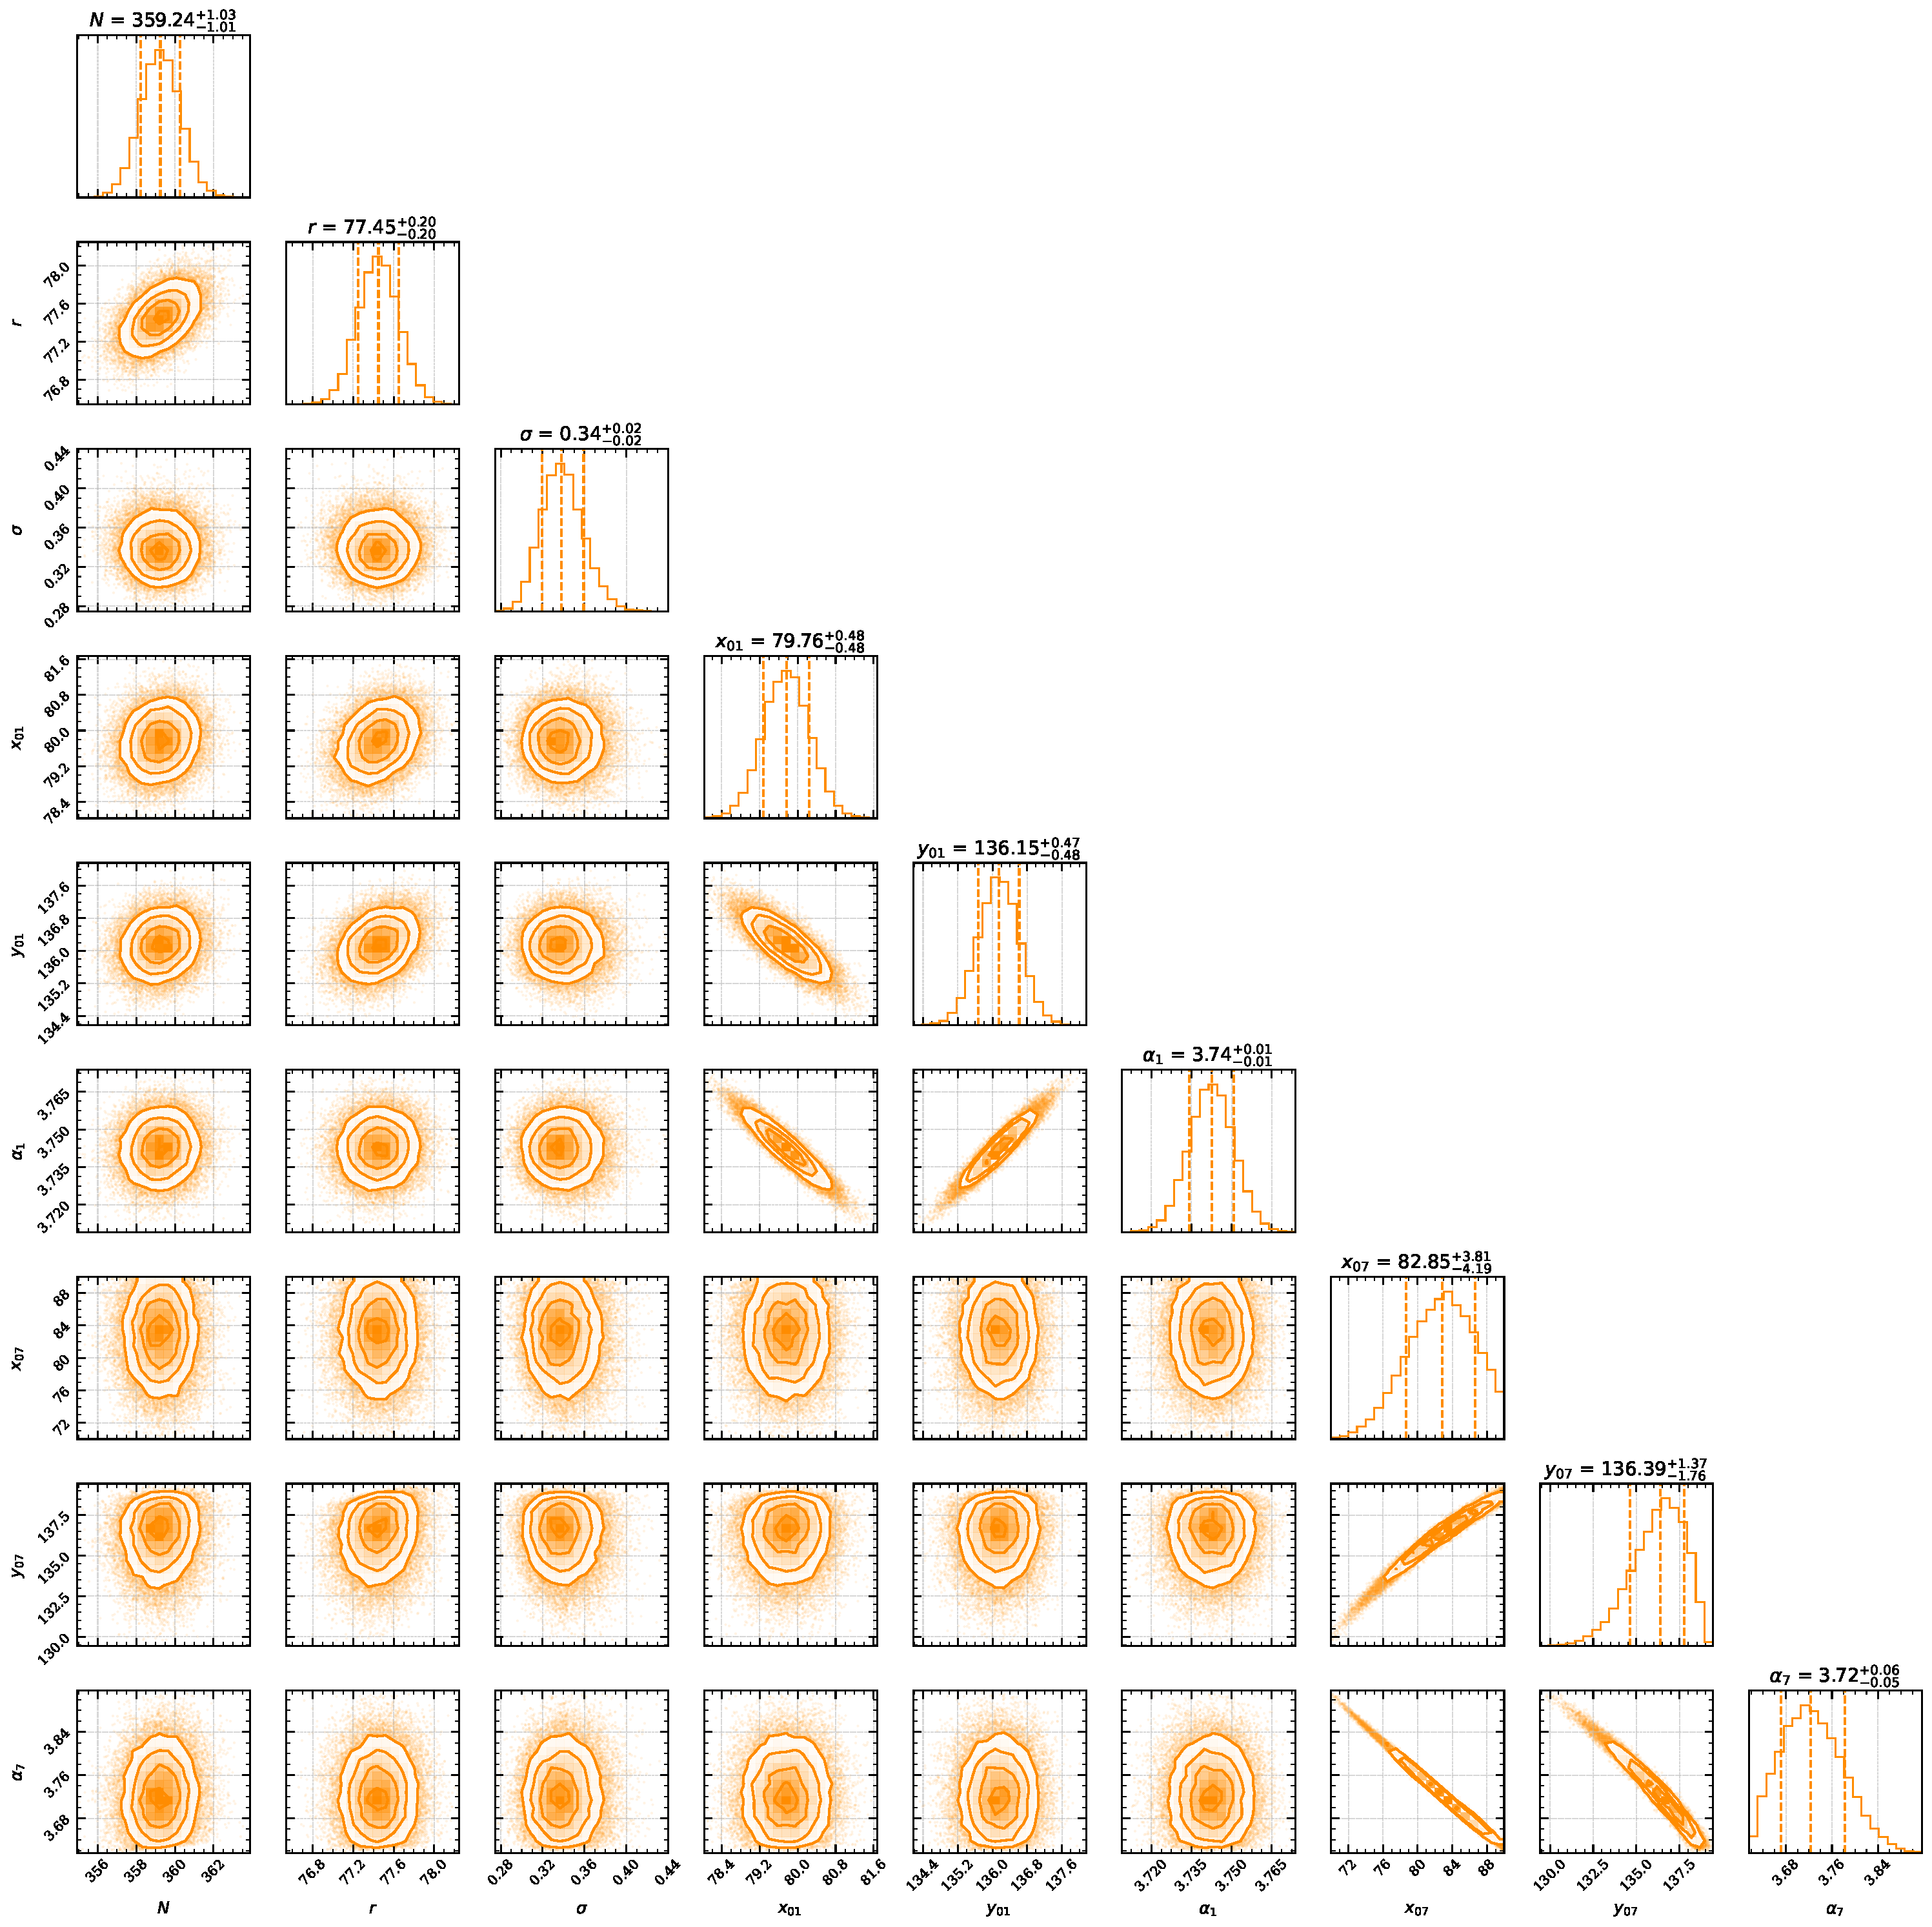
\includegraphics[width=0.99\textwidth]{./figures/corner_plot_isotropic.pdf}
\caption{Corner plot showing posterior distributions and parameter correlations for the isotropic model of the Antikythera mechanism. Key parameters include the total number of holes ($N$), ring radius ($r$), measurement uncertainty ($\sigma$), and section-specific centre coordinates and phase angles for Sections 1 and 7. Diagonal panels show marginalised 1D posterior distributions; off-diagonal panels show joint 2D distributions. Strong correlations are observed between centre coordinates and angular offsets within the same section.}
\label{fig:corner_isotropic}
\end{figure}

\newpage

\begin{figure}[h!]
\centering

\includegraphics[width=0.99\textwidth]{./figures/corner_plot_radial_tangential.pdf}
\caption{Corner plot showing posterior distributions and correlations for the radial–tangential model. Parameters include the total number of holes ($N$), ring radius ($r$), radial and tangential uncertainties ($\sigma_r$, $\sigma_t$), and section-specific centre coordinates and angular offsets for Sections 1 and 7. Compared to the isotropic model (Figure~\ref{fig:corner_isotropic}), this model exhibits weaker correlations between local parameters, suggesting improved identifiability and robustness due to the anisotropic error structure.}
\label{fig:corner_rt}
\end{figure}

\subsection{Comparison}
\label{sec:sd-ratio}
Calculating the posterior odds ratio is an effective way to evaluate competing models. Here, we assume a prior odds ratio of 1, treating both models as equally likely a priori. As we will show, the evidence overwhelmingly outweighs the prior odds, allowing us to focus solely on the evidence ratio, also known as the \textbf{Bayes factor}. This factor serves as a Bayesian analogue to the \textbf{likelihood-ratio test}, but it compares integrated (marginal) likelihoods rather than maximum likelihoods \cite{WikipediaBayesFactor}.

\begin{figure}[h!]
\centering

\includegraphics[width=0.8\textwidth]{./figures/savage_dickey_ratio.pdf}
\caption{Posterior distribution of the log-difference in standard deviations, $\log \sigma_r - \log \sigma_t$, estimated via kernel density from MCMC samples. The shaded region shows the posterior samples; the solid blue curve is the KDE-smoothed posterior density. The vertical dashed line at zero represents the null hypothesis of isotropy (equal variances). The red point indicates the posterior density at this null value, which is nearly zero—implying strong evidence in favour of the anisotropic (radial–tangential) model.}
\label{fig:sd-ratio}
\end{figure}

The \textbf{Savage–Dickey Density Ratio (SDDR)} offers a convenient method for computing Bayes factors when comparing nested Bayesian models. In this analysis, we define \( \theta = \log(\sigma_r/\sigma_t)\), where the null hypothesis \( H_0: \theta = 0 \) corresponds to the isotropic model (equal dispersions), and \( H_1 \) allows for anisotropy.

The Bayes factor in favour of the null hypothesis is given by:
\[
\text{BF}_{01} = \frac{p(\theta = 0 \mid \text{data}, H_1)}{p(\theta = 0 \mid H_1)}
\]
where \( p(\theta = 0 \mid \text{data}, H_1) \) is the posterior density of \( \theta \) evaluated at zero under the alternative model \( H_1 \), and \( p(\theta = 0 \mid H_1) \) is the corresponding prior density at that point.

In our implementation, the posterior density is estimated using kernel density estimation (KDE) from MCMC samples (Figure \ref{fig:sd-ratio}), while the prior density is computed analytically, assuming independent log-uniform priors on \( \sigma_r \) and \( \sigma_t \).

In our case, the posterior density at $\theta=0$ ($\log \sigma_r = \log \sigma_t$) is approximately 0. This implies \textbf{overwhelming evidence against the null hypothesis} \( H_0 \) (the isotropic model) in favour of the alternative: the radial-tangential model.

\paragraph{Prior Density of \texorpdfstring{\( \log(\sigma_r) - \log(\sigma_t) \)}{log(\sigma_r) - log(\sigma_t)} at Zero}

To compute the Savage-Dickey ratio, we require the prior density of \( \log(\sigma_r) - \log(\sigma_t) \) at zero. Let \( U = \log(\sigma_r) \sim \text{Uniform}(a, b) \) and \( V = \log(\sigma_t) \sim \text{Uniform}(c, d) \), where:
\[
a = \log \sigma_{r,\min}, \quad b = \log \sigma_{r,\max}, \quad c = \log \sigma_{t,\min}, \quad d = \log \sigma_{t,\max}
\]
Define \( W = U - V \). The random variable \( W \) thus represents the difference of two independent uniform variables. Its density function \( f_W(w) \) can be derived using convolution:
\[
f_W(w) = \int_{-\infty}^{\infty} f_U(u) f_V(u - w)\, \mathrm{d}u
\]
where \( f_U \) and \( f_V \) are the densities of \( U \) and \( V \), respectively.

This convolution is geometrically equivalent to computing the length of the overlap between the intervals \( [a, b] \) and \( [c + w, d + w] \), scaled by the product of the normalising constants of \( U \) and \( V \). The density becomes:
\[
f_W(w) = \frac{1}{(b-a)(d-c)} \cdot \text{length}([a, b] \cap [c+w, d+w])
\]
At \( w = 0 \), this reduces to:
\[
f_W(0) = \frac{\min(b, d) - \max(a, c)}{(b-a)(d-c)}
\]
Substituting back into terms of the original parameters:
\[
f_W(0) = \frac{\min(\log \sigma_{r,\max}, \log \sigma_{t,\max}) - \max(\log \sigma_{r,\min}, \log \sigma_{t,\min})}{\log(\sigma_{r,\max}/\sigma_{r,\min}) \cdot \log(\sigma_{t,\max}/\sigma_{t,\min})}
\]

In the special case where \(\sigma_r\) and \(\sigma_t\) share identical prior ranges, i.e., \(\sigma_{r,\min} = \sigma_{t,\min}\) and \(\sigma_{r,\max} = \sigma_{t,\max}\), the expression simplifies further to:
\[
f_W(0) = \frac{1}{\log(\sigma_{r,\max}/\sigma_{r,\min})}
\]













\section{Discussion}

\paragraph{Role of Covariance Matrix}
In the literature \cite{woan2024improvedcalendarringholecount}, a Gaussian likelihood is employed to model errors in the measurement and placement of the holes. In a two-dimensional Gaussian error model, the covariance matrix $\Sigma$ characterises the shape, size, and orientation of the error distribution, where the error vector is defined as $\mathbf{e}_i = \mathbf{m}_i - \mathbf{d}_i$. The diagonal elements of $\Sigma$ represent the variances in each direction, while the off-diagonal elements capture the covariances between the error components.

In the simple isotropic model, $\Sigma = \begin{pmatrix} \sigma^2 & 0 \\ 0 & \sigma^2 \end{pmatrix}$, implying that errors are uncorrelated across directions and have the same magnitude in all directions—resulting in circular error contours.

The radial–tangential model, by contrast, decomposes errors into components along the radial direction ($\hat{\mathbf{r}}_{ij}$, pointing from the section centre to the hole) and the tangential direction ($\hat{\mathbf{t}}_{ij}$, perpendicular to the radial direction, following the arc of the ring). It assumes the radial and tangential errors ($e_r$ and $e_t$) are independent as well, but potentially have different magnitudes, allowing for elliptical error contours aligned with the geometry of the ring.


\paragraph{Model Comparison Conclusion}

One might intuitively consider the radial–tangential model a plausible candidate \textit{a priori}. For example, when the holes were originally marked or drilled onto the ring, the precision of the tools used to maintain a constant radius may have differed from the precision needed to achieve equal angular spacing. Intuitively, achieving uniform angular intervals is more difficult, and this directional discrepancy in placement errors may not be negligible.

This intuition is supported by our results: the tangential uncertainty $\sigma_t$ is significantly larger than the radial uncertainty $\sigma_r$ (0.489 vs. 0.040). Visual evidence from Figure~\ref{fig:locations_isotropic} and Figure~\ref{fig:locations_rt} also highlights that error dispersion is more prominent along the tangential direction.

Quantitatively, we implemented a likelihood-ratio test to compare the nested isotropic model with the more general radial–tangential model (Section~\ref{sec:lrt}). The test statistic, $\lambda = 150.94$, far exceeds the critical value of $\chi^2_1 = 10.83$ at the 0.1\% significance level. Additionally, the MCMC analysis in Section~\ref{sec:sd-ratio} employed the Savage–Dickey density ratio, showing that the posterior density at $\theta = \log(\sigma_r/\sigma_t) = 0$ (the isotropic case) is effectively zero. Figure~\ref{fig:sd-ratio} illustrates that the posterior distribution of $\log(\sigma_r) - \log(\sigma_t)$ is centred far from zero.

Taken together, these findings—both frequentist and Bayesian—provide overwhelming statistical evidence against the isotropic model, and strongly support the radial–tangential alternative.

\paragraph{Number of Holes}

Our radial–tangential model estimates the number of holes to be $357.268^{+0.202}_{-0.008}$ (maximum likelihood, 99\% confidence interval), or $358.507^{+3.293}_{-3.142}$ based on MCMC sampling (99\% credible interval). These estimates do not support the hypothesis of a 354-hole lunar calendar. Furthermore, a ring with 365 holes—consistent with a solar calendar—is also strongly disfavoured by our results.



\clearpage
\newpage
\appendix
\section{Use of AI Tools}
In this report, AI tools were utilised to enhance the quality and presentation of the content. Their contributions include:

\begin{itemize}
    \item \textbf{Drafting} – Assisted in writing various sections of the report, particularly some mathematical derivations, as well as parts of the Introduction, Discussion, and Appendix. AI tools were also used to generate captions for figures and tables.

    \item \textbf{Proofreading} – Reviewed grammar, improved sentence structure, and suggested alternative wordings to enhance clarity and coherence throughout the report.

    \item \textbf{LaTeX Assistance} – Helped resolve issues encountered during the LaTeX formatting process, including debugging compilation errors and formatting well-structured tables based on the provided data.
\end{itemize}



\section{Template Information}
This report was formatted using the LaTeX template provided in the Example Coursework by Michal Dorko, with some modifications applied.


\newpage
\printbibliography
\end{document}
